\section{The Dalvik Executable Format}
\label{sec:dex}

The Dalvik virtual machines runs applications stored in the Dalvik executable format. As Android has a Java-based application model, programs are written in a dialect of the Java programming language, and are then compiled to Java bytecode. A tool called \verb|dx| is then used to further compile the .class files into the Dalvik executable format. The Dalvik executable format is designed to be run on devices constained in processor and memory speed.

An Android device with a total of 64 MB system RAM will typically only have 20 MB left over after low-level startup and high-level services have started. This is further reduced to 10 MB of RAM with a large sytem library like Dalvik's\cite{dalvik_int}. The virtual machine, therefore, needs to have a very light memory footprint. Some of the ways in which is achieves this is through the design of the Dalvik executable format, which was designed to be as light-weight as possible. As a result, it is an extremely compact format. An uncompressed Dalvik executable file is around 44\% to 48\% the size of an uncompressed Java .jar file, while a compressed .jar file is around 50\% the size of an uncompressed one\cite{dalvik_int}.

The Dalvik executable file places a huge emphasis on code and data sharing to reduce memory usage. The file structure is broken down at the topmost level by the specification given in Table~\ref{tab:dalvik_layout}:

\begin{center}
\begin{table}[htbp]
    \begin{tabular}{ | l | p{10cm} | } \hline
    Name 		& Description \\ \hline
    header		&	Lists the offsets into the file at which the following sections can be found, as well as additional information about the file. \\ \hline
	string\_ids	&	Lists the strings used by the file, whether used in internal naming or as constant data as used in code. Given in order by string contents. \\ \hline
	type\_ids	&	Lists the type identifiers used by the file (whether classes, arrays or primitives), whether defined in the file or not. Given in order by index into the string\_ids section. \\ \hline
	proto\_ids	&	Lists the method prototypes refered to by the file. Given in order by the return type's index into the type\_ids section. \\ \hline
	field\_ids	&	Lists the field identifiers used by the file, whether defined in the file or not. Given in order by the defining type's index into the type\_ids section. \\ \hline
	method\_ids	&	Lists the methods refered to by the file, whether defined in the file or not (\ie Java standard library functions).
					Given in order by the return type's index into the type\_ids section. \\ \hline
	class\_defs	&	Lists the class definitions, such that a class's superclass and interfaces are listed earlier that the referring class. \\ \hline
	data		&	Data area, which gives support for the items listed above. \\ \hline
	link\_data	&	Data used in statically linked files. \\ \hline
    \end{tabular}
    
    \caption{Layout of Dalvik executable format}
    \label{tab:dalvik_layout}
\end{table}
\end{center}

Examining the file structure of the Dalvik executable format, we can see the methods employed by the Android team to keep the file size as small as possible. The most noticeable of these is the sharing of constant pools. Inside a Java .jar archive, each class definition receives its own heterogeneous constant pool, in which most of the literal constant values are stored. This includes all of the constant sections in the Dalvik executable format such as strings, types and methods. The difference between the two formats is that in the .jar file, each value in the pool is given its own `tag byte' which declares the constant's type. The Dalvik executable format, however, uses per-type constant pools which implicitly give the constant a type, meaning the tag byte can be discarded and thus saving space.

Moreover, the Dalvik executable format amalgamates duplicate constants into one, avoiding repetition of unnecessary data. If two methods were to have the same prototype, the prototype would be listed only once in the Dalvik file. Both method definitions would receive a reference to the same prototype. Additionally, since multiple .class files are compiled into one Dalvik executable file, the elimination of duplicate constants is applied throughout the entire application. The Dalvik executable format favours indirection over repetition. The application-wide sharing of constant pools is shown in Figure \ref{fig:dex}.

\begin{figure}[h!]
    \centering
    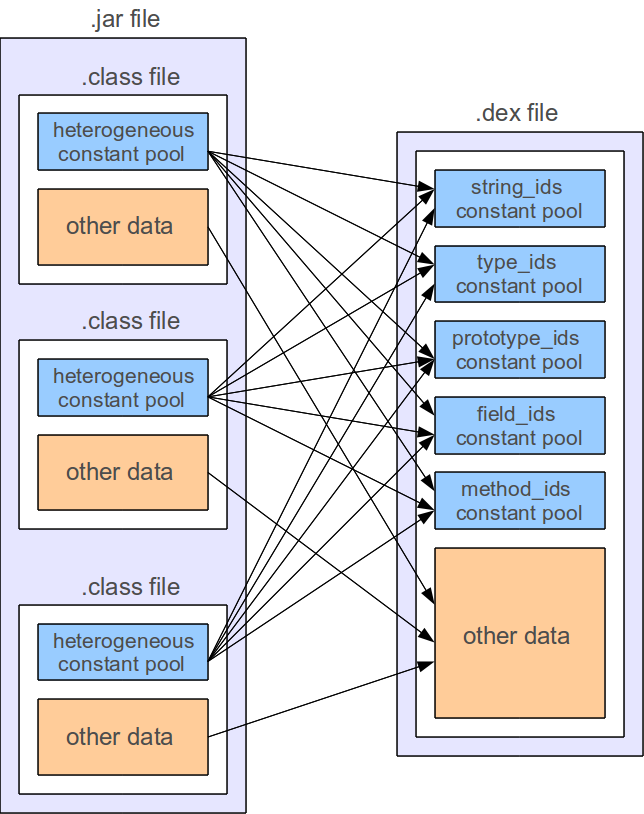
\includegraphics[width=0.8\textwidth]{images/dex.png}
    \caption{Sharing Constant Pools}
    \label{fig:dex}
\end{figure}

